\documentclass[11pt]{article}

\usepackage[margin=1in]{geometry}
\usepackage{amsmath,amssymb,amsthm}
\usepackage{graphicx}
\usepackage[hidelinks]{hyperref}

\newtheorem{theorem}{Theorem}
\newtheorem{corollary}{Corollary}

\newcommand{\R}{\mathbb{R}}
\newcommand{\SL}{\mathrm{SL}}
\newcommand{\GL}{\mathrm{GL}}
\newcommand{\St}{\operatorname{St}}

\title{A Rosenthal-positive unipotent orbit in \(\SL_2(\R)\)}
\author{Run \texttt{fa\_banach\_001}, lane 6}
\date{June 18, 2026}

\begin{document}
\maketitle

\section*{Status}

\textbf{Partial result.}  This packet proves that a natural homogeneous
subspace \(G/H\) of the conjugation \(G\)-space \(G_c\), for
\(G=\SL_2(\R)\), is Rosenthal representable.  It does not decide whether
the whole conjugation action \(G\curvearrowright G_c\) is Rosenthal
representable.

\section*{Source question and context}

The source paper is Michael Megrelishvili, \emph{Topological group
actions by group automorphisms and Banach representations},
arXiv:2110.01386.  The main concrete question asks:

\begin{center}
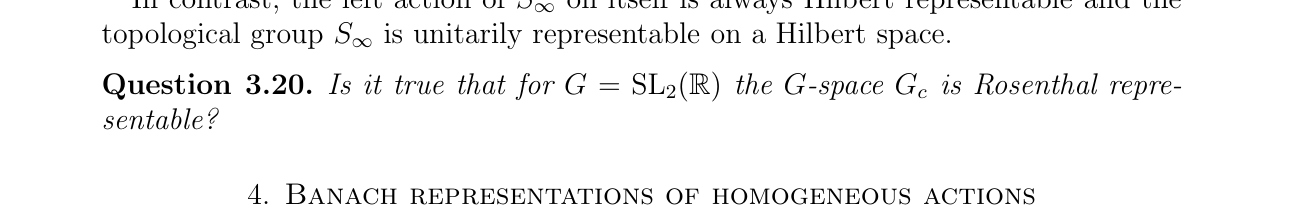
\includegraphics[width=0.96\linewidth]{figures/question_3_20_crop.png}
\end{center}

The same paper observes that the proof of non-reflexive representability
for \(G_c\) already takes place on the unipotent conjugacy orbit of
\[
u=x_1=\begin{pmatrix}1&1\\0&1\end{pmatrix},
\]
and identifies this orbit with a locally compact coset space \(G/H\).
It then asks which homogeneous \(G\)-spaces \(G/H\) are Rosenthal
representable:

\begin{center}
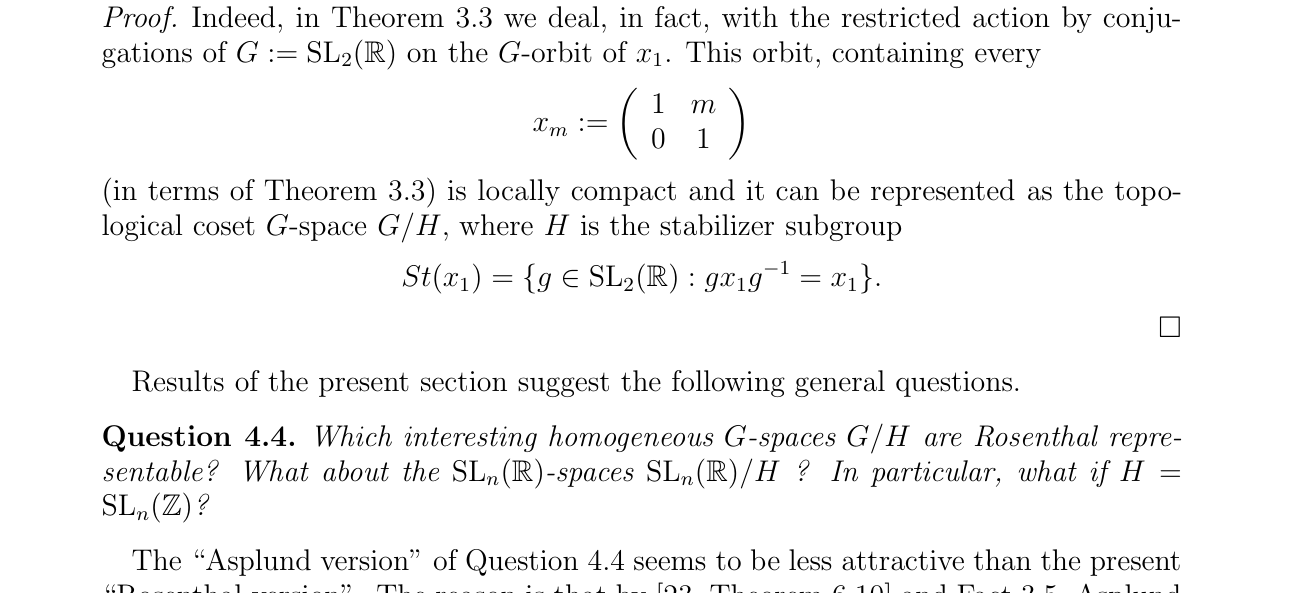
\includegraphics[width=0.96\linewidth]{figures/coset_question_4_4_crop.png}
\end{center}

\section*{Proof Intuition}

The unipotent orbit is not an arbitrary piece of \(G_c\).  It is the
cone of nonzero rank-one nilpotent matrices in \(\mathfrak{sl}_2(\R)\),
translated by the identity.  This cone is parametrized by nonzero
vectors \(v\in\R^2\), up to the sign \(v\sim -v\), through a quadratic
map \(v\mapsto N_v\).

Megrelishvili proves that the one-point compactification of the linear
\(\GL_2(\R)\)-action on \(\R^2\) is tame.  The key observation here is
that the one-point compactification of the unipotent orbit is a
\(\SL_2(\R)\)-factor of that tame compactification: both the zero vector
and the point at infinity are sent to the single added point of the
unipotent orbit compactification.  Tameness passes to factors, hence
the orbit is Rosenthal representable.

\section*{The theorem}

\begin{theorem}
Let \(G=\SL_2(\R)\), let
\[
u=\begin{pmatrix}1&1\\0&1\end{pmatrix},
\]
and let
\[
H=\St(u)=\{g\in G: gug^{-1}=u\}.
\]
Then the homogeneous \(G\)-space \(G/H\), identified with the conjugacy
orbit \(G\cdot u\subset G_c\), is Rosenthal representable.
\end{theorem}

\begin{proof}
Let \(\omega(v,w)=\det(v,w)\) be the standard symplectic form on
\(\R^2\).  For \(v\in\R^2\), define a linear operator
\[
N_v(w)=\omega(v,w)v.
\]
In coordinates \(v=(a,b)\),
\[
N_v=
\begin{pmatrix}
-ab & a^2\\
-b^2 & ab
\end{pmatrix}.
\]
Thus \(N_v\in\mathfrak{sl}_2(\R)\), \(N_v^2=0\), and
\(N_v\neq 0\) for \(v\neq 0\).  Also \(N_{-v}=N_v\), and
\(N_{\lambda v}=\lambda^2N_v\).

For every \(g\in G\), preservation of \(\omega\) gives
\[
gN_vg^{-1}=N_{gv}.
\]
Since every nonzero vector of \(\R^2\) is the first column of some
matrix in \(\SL_2(\R)\), the conjugacy orbit of
\(u=I+N_{(1,0)}\) is exactly
\[
O:=G\cdot u=\{I+N_v:v\in\R^2\setminus\{0\}\}.
\]
This orbit is \(G\)-equivariantly homeomorphic to \(G/H\).

Let \(X=\R^2\cup\{\infty_X\}\) be the Alexandrov one-point
compactification of \(\R^2\), equipped with the natural \(G\)-action.
Let \(Y=O\cup\{\infty_O\}\) be the Alexandrov one-point compactification
of the locally compact orbit \(O\).  Define
\[
q:X\longrightarrow Y
\]
by
\[
q(v)=I+N_v \quad (v\neq 0), \qquad q(0)=q(\infty_X)=\infty_O.
\]
The map is onto and \(G\)-equivariant by the identity
\(gN_vg^{-1}=N_{gv}\).

It remains only to check continuity at the two points collapsed to
\(\infty_O\).  Let \(K\subset O\) be compact.  Since \(O\) is embedded
in the Hausdorff group \(G\), \(K\) is closed in \(G\).  If
\(v_i\to 0\) and \(I+N_{v_i}\in K\), then \(I+N_{v_i}\to I\) in \(G\),
forcing \(I\in K\), impossible because \(I\notin O\).  Hence vectors
sufficiently close to \(0\) are mapped outside \(K\).  Similarly, if
\(\|v_i\|\to\infty\), then the matrix entries of \(N_{v_i}\) are
unbounded, so \(I+N_{v_i}\) eventually leaves every compact subset of
\(O\).  These are precisely the neighborhood conditions for continuity
at \(0\) and at \(\infty_X\).  Thus \(q\) is a continuous
\(G\)-factor map from \(X\) onto \(Y\).

By Theorem 3.12 of \cite{Megrelishvili}, the linear
\(\GL_2(\R)\)-action on \(\R^2\) has tame one-point compactification.
Restricting the acting group from \(\GL_2(\R)\) to \(G=\SL_2(\R)\)
preserves tameness, and tameness passes to compact factors.  Therefore
\(Y\) is a tame compact metric \(G\)-space.  By Fact 3.11 of
\cite{Megrelishvili}, compact metric tame systems are exactly the
systems representable on Rosenthal Banach spaces.  Since \(Y\) is a
proper \(G\)-compactification of \(O\simeq G/H\), the homogeneous
\(G\)-space \(G/H\) is Rosenthal representable.
\end{proof}

\begin{corollary}
For \(G=\SL_2(\R)\), the stabilizer \(H=\St(u)\) gives a homogeneous
space \(G/H\) which is Rosenthal representable but not reflexively
representable.
\end{corollary}

\begin{proof}
Rosenthal representability is the theorem above.  Non-reflexive
representability is exactly the source paper's Corollary 4.3, whose
proof says that Theorem 3.3 works on this restricted conjugacy orbit.
\end{proof}

\section*{Limitations}

This does not settle Question 3.20.  Tameness of a \(G\)-subspace or a
single orbit compactification does not imply tameness of the whole
conjugation \(G\)-space \(G_c\).  The result only shows that the
specific unipotent orbit responsible for the paper's double-limit
non-WAP argument cannot also serve as a non-Rosenthal witness.

\section*{Novelty and literature check}

Local run indexes were searched for arXiv id \texttt{2110.01386}, the
title, \(\SL_2(\R)\), Rosenthal representability, unipotent orbit, and
the stabilizer notation \(St(x_1)\); no duplicate packet or attempt was
found.  Web searches on June 18, 2026 used exact combinations of
\(\SL_2(\R)\), Rosenthal representability, \(St(x_1)\), unipotent
orbit, and Megrelishvili.  They found the source paper but no later
resolution or prior statement of this factor-map consequence.

\begin{thebibliography}{9}

\bibitem{Megrelishvili}
M. Megrelishvili,
\emph{Topological group actions by group automorphisms and Banach
representations},
Forum Mathematicum, accepted version; arXiv:2110.01386, 2023.

\end{thebibliography}

\end{document}
